\documentclass[envcountsame,envcountchap,letterpaper]{svmono}
\usepackage{makeidx}
\usepackage{amsmath}
\usepackage{amsfonts}
\usepackage{amssymb}
\usepackage{graphicx}
\usepackage[bottom]{footmisc}
\usepackage{hyperref}
\usepackage{color}
\usepackage{float}
\usepackage[brazilian]{babel}
\usepackage[utf8]{inputenc}

\hypersetup{colorlinks=true, linkcolor=black, citecolor=black, urlcolor=black}

\makeindex

\author{Hildeberto Mendonça \\ Manoel Calixto}
\title{Yougi}
\subtitle{Gerindo o Conhecimento Produzido pela Comunidade}
\begin{document}

\maketitle

\frontmatter

\thispagestyle{empty}
\vspace*{3.5cm}
\begin{flushleft}
Aviso: cópias deste documento pode ser feita para o seu uso próprio e para distribuição para outros, desde que você não cobre qualquer taxa por essas cópias e desde que cada cópia contenha este aviso de copyright, distribuído em papel ou eletronicamente.
\end{flushleft}

\tableofcontents

\listoffigures

\listoftables

\mainmatter

\chapter{Introdução}

\section{O que é um User Group?}

\section{Caso de Estudo}

O estudo de caso escolhido é baseado na experiência pessoal da equipe que Você está desenvolvendo. A maioria das contribuições são provenientes do Cear\'{a} Java User Group, que é um grupo de usuários técnicos localizados na costa Nordeste do Brasil. Apesar de ser parte de um domínio específico, acreditamos que o modelo proposto é genérico o suficiente para cobrir as necessidades da administração da maioria dos user groups lá fora.

\subsection{O Cenário do Java User Group}

Java User Groups (JUG) são comunidades independentes de empresários, estudantes e profissionais em torno da plataforma Java e tecnologias relacionadas. Eles estão espalhados globalmente com maior concentração na Europa, América do Norte e América do Sul.

A sua independência da indústria é particularmente interessante porque, em geral, grupos de usuários são promovidas pela indústria, que é o caso do GUG, ligado a Google; OUG, ligado a Oracle; e MUG, ligado a Microsoft.

\subsection{JUGs Ao Redor do Mundo}

\subsection{A Necessidade de um gerenciador maduro para User Group}

\section{Yougi Missão e Visão}

Yougi é desenvolvido por pessoas apaixonadas pelo o que fazem, diariamente por vários anos, o que a aplicação faz hoje é o que está planejado para fazer amanhã para comunidades online lá fora. Depois de dois anos de desenvolvimento contínuo, Yougi consolidou sua missão de gerir, promover e difundir o conhecimento produzido por uma comunidade de membros que partilham os mesmos interesses e paixões.

O projeto vai além de serviços para as comunidades e estende o seu impacto em outras áreas como a educação, competividade econômica e geração de oportunidades. Como a plicação é disponibilizada como software livre e aberto, várias questões técnicas da lista de discussão do CEJUG são realmente abordadas por exemplos extraídos a partir do código-fonte do Yougi. Iniciantes e profissionais aprendem a programar e usar a plataforma de estudando como a aplicação foi desenvolvida.

\section{Visão Geral}

\section{Convenções usadas neste livro}

\part{Guia do Usuário}

\chapter{Gerenciamento de Membros}

\section{Inscrição}

A decisão de se cadastrar no users group sempre deve vir da pessoa interessada. E por isso que a única maneira de adicionar um novo membro é preencher o formulário de inscrição inicial acessível através de um link no cabeçalho da aplicação quando nenhum membro estiver logado.

Além dos dados pessoais básicos, o formulário de inscrição também pede à pessoa interessada para selecionar uma ou mais das seguintes opções:

\begin{itemize}
\item ``Eu quero estar ciente de todos os eventos organizados e apoiados pelo UG em um nível local, nacional e internacional'' - como membro, a pessoa vai receber informações sobre eventos organizados pelo o UG (consulte o Capítulo \ref{chp:event-management}) e outros eventos apoiados, promovido por parceiros e patrocinadores.

\item ``Quero receber de patrocinadores' e parceiros' ofertas de produtos e serviços, como livros, cursos, revistas, etc'' - apenas os membros que marcarem esta opção irá participar de sorteios, promoções e outros concursos promovidos por patrocinadores.

\item ``Quero receber ofertas locais e nacionais de trabalho relacionadas com Java'' - apenas os membros que marcarem esta opção irá receber as ofertas de trabalhos de parceiros e patrocinadores.

\item ``Quero participar da lista de discussão técnica'' - Marcando esta opção, o membro será automaticamente registrado na lista de discussão técnica.

\item ``Quero receber notícias sobre Java e outras tecnologias relacionadas, bem como notícias sobre o mercado e outras comunidades'' - apenas os membros que verificarem esta opção irá receber notícias sobre assuntos discutidos no grupo e outras atividades comunitárias.

\item ``Outros membros do UG serão capazes de ver o meu perfil e me contatar diretamente através da aplicação. O aplicativo irá proteger cuidadosamente o endereço de e-mail, não mostrando para os outros'' - apenas membros que marcarem esta opção será capaz de usar os recursos sociais da aplicação.
\end{itemize}

Quando a pessoa interessada envia o formulário de inscrição, nós temos que ter certeza de que o seu endereço de e-mail está correto antes de o considerar como um membro. Enviamos um e-mail para o endereço de e-mail informado no formulário, pedindo que a pessoa interessada confirme o seu endereço de e-mail, clicando no link de confirmação. Este link contém um código único, que garante que o link não pode ser reutilizado após seu primeiro uso, confirmando o endereço de e-mail apenas uma vez. A pessoa interessada é considerada como um membro tão logo o seu endereço de e-mail é confirmado. O novo membro recebe uma mensagem de e-mail de boas-vindas e os Líderes do JUG são informados por e-mail sobre a inscrição com sucesso do membro.

\section{Perfil do Usuário}

O membro tem o direito de ler e modificar os dados publicados no seu próprio perfil. O endereço do e-mail é somente para validar os dados. A validação de e-mail funciona da mesma maneira que funciona durante a inscrição: o sistema envia uma nova mensagem para o endereço de e-mail, com um código de confirmação para validá-lo.

\section{Desativação}

A desativação de um membro significa que ele não vai participar das atividades do grupo a partir da data da desativação. Nenhuma mensagem de e-mail, convite, oferta, ou qualquer outro tipo de informação será enviada ao membro desativado nunca mais. Portanto, ele não é considerado como um membro regular.

Ao mesmo tempo, toda a entrada de dados por parte do membro antigo na base de dados não serão removidas. Comentários, e-mails, artigos e outras informações será mantida inalterada indefinidamente. Portanto, qualquer modificação sobre esses dados não é responsabilidade da aplicação.

\chapter{Gerenciamento de Eventos}
\label{chp:event-management}

Eventos são estratégicos para user groups e para as empresas que querem promover o uso de sua tecnologia ou atrair pessoas de talento para compor sua equipe dos sonhos. A ocasião é apropriada para disseminar o conhecimento e promover o networking, o reforço dos laços entre as pessoas e aumentando a probabilidade de novas oportunidades. Atualmente, existem várias maneiras de construir um network virtualmente, mas a linguagem corporal ainda é a maneira mais eficiente de conhecer o comportamento das pessoas, confiabilidade e simpatia. Those good experiences Good ex

É importante ter uma gestão de eventos eficiente, a fim de manter tudo sob controle, mensurar a participação dos membros e obter seus feedbacks.

\section{Inscrição no Evento}

Para começar a organizar os eventos, Os Líderes do UG deve registrar locais disponíveis e adequados para eventos do user groups. Um local pode ter um ou mais salas onde as sessões do evento acontecerá. Em caso de ter várias salas disponíveis, o evento pode gerenciar múltiplas sessões em paralelo.

Os eventos são alocados em locais já existentes para um determinado período de tempo. Quando um evento é registrado e atribuído a um local, o local é contatado recebendo um e-mail contendo os detalhes sobre o evento e uma lista de recursos que se espera deles. Depois de um processo de negociação o evento é confirmado ou não. A confirmação ocorre quando o local clica no link de confirmação na mensagem de e-mail. Sem essa confirmação o evento não pode ocorrer.

Para cada sessão do evento, um ou mais palestrantes podem ser alocados. Um palestrante é uma pessoa qualificada sobre o(s) assunto(s) da sessão. Ele é convidada por um líder do UG para dar uma palestra, treinamento, coordenar uma discussão ou qualquer outra atividade social. A pessoa é convidada a se registrar na aplicação como um palestrante. Uma vez conectado, ele pode colocar um breve resumo de sua experiência, um resumo da sessão, fazer upload da sua foto para o perfil, apresentações, documentos, código fonte, links e outros conteúdos úteis para a sessão. A aplicação vai usar todas essas informações para compor a página do evento.

Quando o evento é confirmado, uma mensagem de e-mail que contém informações detalhadas é enviado a todos os membros que declararam em sua ficha de inscrição o desejo de receber informações sobre os eventos. Esta mensagem contém um link direto para o formulário de inscrição do evento.

Informações detalhadas sobre o evento também é formatado para ser publicada no site da UG. Consequentemente, isso pode atrair pessoas que estão interessadas no evento, mas não são membro da UG. Essas pessoas devem se tornar um membro da UG antes de se inscrever para o evento.

Logo após o registro no evento, o membro recebe uma mensagem de confirmação apenas para que ele ficar sabendo que está registrado com êxito para participar do evento. Membros registrados receberão uma mensagem lembrete de e-mail, sete dias antes do evento e um segundo no dia antes do evento. Eles podem cancelar sua inscrição a qualquer momento antes do evento.

\section{Controlando o evento}

Na entrada do evento, um membro do pessoal do UG verifica a inscrição de cada pessoa em um computador disponível. Se a pessoa for um membro inscrito no evento, em seguida, sua presença está confirmada. Se a pessoa é um membro, mas ele não está inscrita no evento, então a seu registro é feito na entrada. Se a pessoa não é um membro, em seguida, ele deve concordar em se tornar um membro do UG, caso contrário não é possível participar do evento. Se ele concorda em se tornar um membro, a inscrição dele no UG e no evento é feita na entrada do evento.

\section{Após o evento}

Quando o evento já passou, não há informações sobre o evento que podem ser alteradas. Ele estará disponível apenas em modo de somente leitura a partir do dia seguinte. Os Palestrantes não serão capazes de atualizar seus perfis até serem alocados para outro evento. No entanto, os líderes do UG são capazes de publicar recursos adicionais relacionados ao evento, como fotos, documentos, apresentações, etc.

\chapter{Gestão de Parceiros}

\section{Inscrição de Parceiros}

\section{Patrocinadores}

\section{Serviços exclusivos para Parceiros}

\subsection{Divulgação de Ofertas de trabalho}

\subsection{Ofertas de Produtos e Serviços}

\subsection{Pesquisa para Pessoas Talentosas}

\chapter{Gestão do Conhecimento}

\section{Tópicos no Âmbito do User Group}

\section{Gestão da listas de discussão}

\section{Agregação de Conteúdo Web}

\part{Guia Técnico}

\chapter{Arquitetura}

Yougi deve ser implantado em um Servidor de Aplicação (SA). Esta plataforma é responsável pela execução do sistema, a conectividade com diversos recursos disponíveis no ambiente e a disponibilidade para vários usuários e sistemas. No momento, o Glassfish 3.1.2 é o padrão de SA para esta aplicação. Este Servidor Java EE ganhou muita atenção por sempre correr para o estado-da-arte da tecnologia do lado do servidor do Java. Tem um roteiro agressivo, sendo sempre o primeiro produto no mercado para implementar totalmente a última versão da especificação do Java EE.

Uma das principais vantagens da utilização de um servidor de aplicações, como o Glassfish é manter o aplicativo livre de código complexo, tal como a) controle manual de transações do banco de dados; b) configuração de acesso de banco de dados; c) segurança de autenticação e autorização; e) envio e recebimento de mensagens de correio eletrônico, entre muitas outras complexidades que são requisitos não-funcionais, consumindo o tempo que seria gasto em requisitos funcionais.

Nenhum teste foi realizado em outros SA até agora, principalmente porque quando o projeto Glassfish começou foi o único SA a implementar a especificação do Java EE 6 (JPA, EJB, JSF, etc.). O SA devem ter acesso e fornecer os seguintes recursos:

\begin{itemize}
\item \textit{Servidor de Banco de Dados}: um driver de banco de dados permite conexões a um banco de dados relacional e um pool de conexão que gerencia várias conexões simultâneas para esse banco de dados, permitindo escalabilidade e desempenho. MySQL é o sistema de banco de dados escolhido para organizar e proteger os dados dos UG's.

\item \textit{Servidor de e-mail}: O serviço do JavaMail se conecta a um servidor de e-mail e fornecer sessões para a aplicação, permitindo que ele enviar e receber mensagens de e-mail sem qualquer configuração especial no lado de implementação.

\item \textit{Security Realm}: é um provedor de dados de autenticação e autorização para identificar os usuários que desejarem acessar o aplicativo e verificar se eles têm direitos de acesso aos recursos protegidos. A aplicação de banco de dados, além de armazenar os dados dos UGs, também armazena os usuários e seus papéis, o que torna o provedor realm, referenciado pelo o Glassfish na configuração do realm.

\item \textit{Sistema de Arquivo}: a aplicação deve ser capaz de salvar e acessar arquivos de um diretório específico do sistema de arquivos. Infelizmente, o SA não gerenciar o acesso ao sistema de arquivos. O aplicativo é responsável por gerenciar todos os arquivos enviados.
\end{itemize}

Os recursos fornecidos pelo servidor de aplicação ajudam a simplificar a arquitetura geral da aplicação. A conectividade com esses recursos caracteriza uma arquitetura de n camadas, onde cada camada é fisicamente separadas. A arquitetura da aplicação, por sua vez, é dividida em quatro camadas, conforme ilustrado na Figura 1. Essas camadas fornecem um modelo para criar uma aplicação flexível e reutilizável. Desta forma, novas funcionalidades podem ser acomodadas de forma eficiente, com um impacto mínimo sobre o código existente.

As 4 camadas lógicas são:

\begin{itemize}
\item \textit{Visão}: implementa a interface do usuário, definindo o layout das telas, posição dos componentes de interface do usuário, realizando a validação de dados (por exemplo, formato de data inválido), formatação de dados a ser apresentado, internacionalização e localização de texto e dar feedback sobre a interação do usuário.

\item \textit{Controlador}: controla o fluxo da navegação de acordo com a interação do usuário e intermedia os dados da camada de visão para a de negócio e vice-versa. Realiza a validação das regras de negócio (por exemplo, usuário já existe), conversão de dados amigável ao usuário para as regras de negocio no modelo e vice-versa, acessar os serviços de negócio, criar objetos dos modelos que não existem ainda e manipula os já existentes. De acordo com o estado da IS, o controlador sabe que o fluxo deve ser seguido e o que fazer em caso de exceções e limitações de segurança.

\item \textit{Negocio}: devido à sua objetividade, a camada de negócios não é subdividida. Considera-se como concreta e está irá executar operações de negócios transacionais em relação ao modelo de dados. Cada operação do negócio deve garantir que o modelo de dados é consistente antes e após a sua execução. Por isso, o modelo de dados só podem ser acesso através desta camada.

\item \textit{Persistência}: Mapeia as entidades do modelo de os com tabelas de banco de dados para gerenciar o ciclo de vida de objetos da entidade. Esses objetos podem ser criados (inserir), atualizado (atualização), consultado (consultar) e excluídos (excluir). Estas operações são largamente utilizados pela camada de objeto de acesso de dados, a fim de interagir com a base de dados. A camada de persistência pode gerenciar uma ou mais fontes de dados, mas uma fonte de dados é gerida por uma única fonte de dados.
\end{itemize}

\section{Tecnologias Escolhidas}

Tabela \ref{tab:chosen-technologies} de lista as tecnologias adotadas pela equipe de desenvolvimento para implementar o aplicativo.

\begin{table}
\centering
\caption{Tecnologias escolhidas para implementar as camadas lógicas}
\label{tab:chosen-technologies}
\begin{tabular}{lll}
\hline\noalign{\smallskip}
Camada de lógica & Tecnologia & Versão \\
\noalign{\smallskip}\hline\noalign{\smallskip}
Visão & JSF Facelets & 2.1 \\
 & Primefaces UI Library & 2.4.2 \\
\noalign{\smallskip}
Controlador & Primefaces & 2.1.1 \\
 & JSF Managed Beans & 2.1 \\
\noalign{\smallskip}
Negócio & EJB Session Beans & 3.1 \\
 & EJB Timer & 3.1 \\
\noalign{\smallskip}
Persistência & JPA & 2.0 \\
 & EclipseLink & 2.0 \\
 & JTA & 1.2 \\
\noalign{\smallskip}\hline
\end{tabular}
\end{table}

Estas tecnologias foram selecionadas com base nas necessidades atuais, recursos e conhecimentos da equipe de desenvolvimento. Decidimos adotar uma abordagem minimalista, onde a maioria das libs necessárias para o aplicativo também são distribuídos com o SA, como o Eclipse Link e Mojarra, e a maioria das configurações são feitas através do console administrativo, tais como o pool de conexão do banco de dados, JavaMail Session e o Security Realm. Para o momento, só a biblioteca externa é a de componentes do Primefaces. Nós fazemos uso extensivo de anotações e evitamos, tanto quanto podemos XMLs para fins de configuração. As operações são totalmente gerenciado pelo contêiner. Dessa forma, mantemos o foco no código fonte do modelo da comunidade do UG. Eventualmente, outras tecnologias fora desta tabela podem ser adotadas se bem justificadas. Portanto, uma nova tecnologia seria considerada no caso de necessidade de um UG muito especial deve ser cumprida.

Entraremos em detalhes sobre as tecnologias escolhidas, descrevemos cada uma delas, descrição completa na Figura 1:

\begin{itemize}
\item \textbf{JSF 2.1}: A tecnologia Java Server Faces é a tecnologia padrão para desenvolvimento de web aplicações na plataforma Java EE.
   \begin{itemize}
   \item \textit{Primefaces}: biblioteca extensiva de Widgets UI 
   disponíveis para a tecnologia JSF.
   \item \textit{Converters}: converte os dados de usuário amigável compatível com o modelo da camada de negócio e vice-versa. 
   \item \textit{ManagedBeans}: classes POJO anotadas que têm
   acesso a recursos especiais disponíveis no
   contexto de aplicação.
   \item \textit{Validators}: executa no lado do servidor a validação de dados informados pelo usuário antes de seguir no processamento do controlador.
   \end{itemize}
\item \textbf{JNDI}: o Java Naming and Directory Service ajuda a localizar e recuperar instâncias de recursos disponíveis no contexto do servidor, reutilizando as instâncias existentes e evitando a complexidade por trás da criação dessas instâncias.
\item \textbf{EJB 3.1}: Modelo de componente transacional, distribuido e seguro para encapsular o lógica de negócio reusável.
   \begin{itemize}
   \item \textit{Stateless Session Beans}: EJB que não armazena o estado dos componentes na memória, otimiza a locação de memória e escalabilidade em vários servidores.
   \item \textit{Timer}: EJB capaz de agendar a
    execução a lógica de negócios em um determinado tempo ou em um
    frequência de tempo determinado. A programação de rotinas é
    muito apropriado para realizar a manutenção automática
    de tarefas como a limpeza de dados temporários, gerar
    relatórios complexos, o envio de mensagens de alerta, etc Timers
    são também úteis para usar eficientemente recursos computacionais
    quando os sistemas estão em modo de espera.
   \item \textit{ManagedBeans}: classes POJO anotadas que têm
    acesso a recursos especiais disponíveis no contexto empresarial.
   \end{itemize}
\item \textbf{JPA 2.0}: Java Persistence API é uma especificação de mapeamento de entidade relacional que gerencia o ciclo de vida de objetos persistentes no banco de dados. Que reduz o grau de dependência de banco de dados, a complexidade do código fonte e o custo de manutenção, no caso de alterações no modelo relacional.
   \begin{itemize}
   \item \textit{Entity Model}: classes POJO anotadas que faz o mapeamento das tabelas do banco de dados, onde suas instâncias representam os registros da tabela para a lógica de negócios.
   \item \textit{JTA}: O Java Transaction API.
   \end{itemize}
\end{itemize}

\section{Modelo do Banco de Dados}

\begin{figure}
\centering
\includegraphics[height=10cm, angle=90]{figures/relational-model}
\caption{Database relational model}
\label{fig:relational-model}
\end{figure}

\subsection{Liquibase}

Para manter o modelo de banco de dados atualizado, Yougi utiliza o Framework Liquibase\footnote{Liquibase. Gerenciador de alterações no banco de dados.  http://www.liquibase.org.}. Esse framework habilita a aplicação para atualizar o banco de dados durante o tempo de implantação. Isso simplifica a atualização da aplicação, reduzindo-a a uma simples implantação.

Durante o tempo de desenvolvimento, Se o banco de dados precisar ser alterado, o desenvolvedor deve adicionar conjuntos de alterações para um ou vários arquivos xml localizado no módulo yougi-web, em src/main/resources/org/cejug/yougi/db/changelog.

\chapter{Instalação}

Para instalar o Yougi nós precisamos de:

\begin{itemize}
\item Java Standard Edition JDK 7;
\item Glassfish 3.1.2 Server ou superior;
\item MySQL 5 ou superior;
\item MySQL ConnectorJ JDBC Driver;
\item acesso para um servidor SMTP e POP 3 para enviar e receber 			  mensagens de e-mail.
\end{itemize}

A instalação inicial leva algum tempo, mas vai garantir atualizações fáceis quando novas versões que sair. Como a instalação do Java SE JDK, Glassfish e MySQL são dependentes de plataforma, nós consideramos que eles já eram desempenhadas pelo administrador, que sabe detalhes sobre o sistema da hospedagem. Não seria completa e atualizada o suficiente aqui, portanto, a melhor fonte de informação é seus respectivos sites. Os passos para instalar a aplicação são:

\begin{enumerate}
\item Crie um banco de dados MySQL: rode os scripts SQL para criar um banco de dados e sua estrutura dedicada para a aplicação. A última versão disponível do script de banco de dados é mysql-create.sql.
\item Instale o Driver JDBC no Glassfish: faça o MySQL ConnectorJ JDBC Driver disponível no classpath do servidor de aplicação para ser usado pelo o pool de conexões para criar novas conexões no banco de dados MySQL.
\item Criar um pool de conexões de banco de dados no Glassfish: ele gerencia o pool de conexão ao banco de dados usando o JDBC Driver.
\item Crie uma fonte de dados para o pool de conexão no GlassFish: a fonte de dados liga o pool de conexão a aplicação. Em outras palavras, o pool de conexão é o recurso e a fonte de dados é um nome para o recurso. Esse nome é usado pela a aplicação para localizar e usar o recurso.
\item Crie um Security Realm: o security realm permite a implementação declarativa de segurança do aplicativo, reduzindo significativamente a complexidade da aplicação, delegando essa responsabilidade para o container.
\item Crie um JavaMail session: pois esse aplicativo lida com as pessoas, tem que enviar e-mails com muita frequência. Portanto, a disponibilidade de um JavaMail session, gerenciado pelo contêiner, é essencial para apoiar a alta demanda de envio e recebimento de e-mails sem lidar com a complexidade de gerenciar as conexões do servidor de e-mail.
\item Implantar o pacote de aplicativos: finalmente, implantar o pacote de aplicativo que faz uso de todas as configurações acima.
\item Configurar a aplicação de acordo com as necessidades específicas do UG: após a implantação inicial do aplicativo será executado normalmente usando a configuração padrão. No entanto, a aplicação estará totalmente operacional apenas quando as configurações específicas para o UG são definidos.
\end{enumerate}

\section{Criando um banco de dados MySQL}

Yougi tem acesso a apenas um banco de dados. Este banco de dados é criado usando o console administrativo e um script SQL. Como mencionado antes, estas instruções consideram que o banco de dados MySQL, versão 5.0 ou superior, já está instalado e configurado. Em termos de configuração, também consideramos que o caminho do sistema operacional está apontando para a pasta onde todos os comandos MySQL localizados.

O procedimento começa a execução do console administrativo, usando o seguinte comando:

\begin{verbatim}
# mysql -u root -p
\end{verbatim}

Geralmente, um usuário administrativo é necessário para criar um novo banco de dados. o usuário \textit{root} é o que tem privilégios para realizar esta operação. Ele vai criar uma sessão de cliente autenticado para acessar o MySQL. \textit{-u} significa que o valor subsequente é o usuário da sessão e \textit{-p} significa que a senha deve ser solicitado logo após a execução do comando. Uma vez autenticado, o utilizador \textit{root} vai permitir a execução do comando abaixo, o que cria a base de dados e um utilizador específico para ele:

\begin{verbatim}
mysql> create database ug;
mysql> create user ug_user identified by '[password]';
mysql> use ug;
mysql> grant all privileges on ug.* to ug_user@'%';
mysql> flush privileges;
\end{verbatim}

O banco de dados \textit{ug} e o usuário \textit{ug\_user} são criados, e todos os privilégios sobre o banco de dados \textit{ug} são concedida ao \textit{ug\_user}. Para verificar se o banco de dados foi criado, execute o seguinte comando:

\begin{verbatim}
mysql> show databases;
\end{verbatim}

Verifique se o banco de dados \textit{ug} se encontra na lista. Então nós temos que sair da sessão root e abrir uma nova sessão para o novo usuário para criar a estrutura de banco de dados. Siga a sequência de comandos abaixo:

\begin{verbatim}
mysql> quit;

# mysql -u ug_user -p

mysql> use ug;
mysql> source [caminho para o script do banco de dados]/mysql_create.sql;
mysql> quit;
\end{verbatim}

O usuário \textit{ug\_user} e a sua senha deve ser usado na configuração do pool de conexão. Não use o usuário \textit{root} para fins de aplicação.

O arquivo \textit{mysql\_create.sql} está disponível dentro do código fonte. Ele está localizado na pasta /yougi-ejb/src/main/resources/META-INF/. Para obter o código-fonte, siga as instruções descritas na seção \ref{ssec:obtaining-source-code} ou obtê-lo na internet no: https://github.com/htmfilho/yougi.

\section{Instalando o Driver JDBC no Glassfish}

A instalação do driver consiste em salvar o arquivo do driver em uma determinada pasta de libs do SA. Para este passo as instruções considerar que o SA Glassfish, é a versão 3.1 ou superior, já está instalado e configurado. O driver está disponível para download no site do MySQL (http://www.mysql.com). O arquivo baixado contém o driver e sua documentação. copie o arquivo do driver, mysql-connector-java-[version]-bin.jar, para a pasta [glassfish\_home]/glassfish/domains/domain1/lib/. Reinicie o SA para tornar o driver disponível.

\section{Crie um Pool de Conexão para o banco de dados}
\label{sec:creating-database-connection-pool}

O pool de conexões do banco de dados é gerenciado pelo SA. Há muitas maneiras de criar um pool de conexões. Nós vamos mostrar duas possibilidades: mudar os arquivos de configuração diretamente e usando o console administrativo.

Para criar o pool de conexão com o banco através do arquivo de configuração, abra o arquivo [glassfish\_home]/glassfish/domains/domain1/config/domain.xml. Ir para o elemento \textless resources\textgreater \ e adicionar o seguinte pool de conexão e de recursos jdbc sob o último elemento de fechamento \textless /jdbc-connection-pool\textgreater \ .

\begin{verbatim}
<resources>
   ...
   </jdbc-connection-pool>
   <jdbc-connection-pool driver-classname="" datasource-classname=
       "com.mysql.jdbc.jdbc2.optional.MysqlConnectionPoolDataSource"
       res-type="javax.sql.ConnectionPoolDataSource" description="" 
       name="UGPool" ping="true">
         <property name="User" value="ug_user"></property>
         <property name="DatabaseName" value="ug"></property>
         <property name="Password" value="password_here"></property>
         <property name="ServerName" value="localhost"></property>
         <property name="PortNumber" value="3306"></property>
   </jdbc-connection-pool>
   <jdbc-resource pool-name="UGPool" description="" 
                  jndi-name="jdbc/ug"></jdbc-resource>
</resources>
\end{verbatim}

Agora, encontre o elemento \textless server name=''server'' config-ref=''server-config''\textgreater \ e colocar dentro do seguinte linha após o último elemento \textless /resource-ref\textgreater :

\begin{verbatim}
<server name="server" config-ref="server-config">

...
<resource-ref ref="jdbc/ug"></resource-ref>
</server>
\end{verbatim}

Se preferir fazê-lo no console administrativo, você pode seguir os passos a seguir:

\begin{enumerate}
\item  Digite no console administrativo em http://[nome-do-servidor]:4848/ e navegue até Resources / JDBC / Connection Pools.
\item Criar um novo pool de conexão com o nome UGPool, selecione o resource type javax.sql.ConnectionPoolDataSource, o vendor do banco de dados MySQL e clique em next.
\item Selecione o datasource classname \\ \textit{com.mysql.jdbc.jdbc2.optional.MysqlConnectionPoolDataSource} e informar as seguintes propriedades:
   \begin{enumerate}
   \item DatabaseName=ug
   \item User=ug\_user
   \item Password=put\_the\_password\_here
   \item PortNumber=3306 (esta é a porta padrão, mas certifique-se
    que você está usando a correta)
   \item ServerName=[nome do servidor ou endereço de IP]
   \end{enumerate}
\item Clique em \textit{Finish} para o novo pool de conexões.
\item Vá para a lista de pools de conexão novamente e selecione o novo que acabou de ser criada.
\item Clique em \textit{Ping} para verificar se a conexão foi configurado corretamente. a mensagem "Ping Succeeded" significa que a ligação está a funcionar bem e pronto para ser utilizado.
\end{enumerate}

Agora, vamos criar um nome JNDI por isso vá \textit{Resources/JDBC/JDBC Resources}.

\begin{enumerate}
\item Clique em \textit{New} para iniciar a criação do data source.
\item Defina o campo \textit{JNDI Name} para \textit{jdbc/ug}.
\item Selecione o pool de conexão \textit{UGPool} (consulte a seção \ref{sec:creating-database-connection-pool}).
\item Clique \textit{Ok} para finalizar.
\end{enumerate}

A única informação que a aplicação sabe sobre o banco de dados é o nome jndi do jdbc, que é ''jdbc/ug''. Isto é importante porque o aplicativo não deve conter todos os dados relacionados à segurança, tais como nome de usuário e senha do banco de dados. Devemos deixar que o administrador do servidor definir estas configuração no servidor, de acordo com seus princípios de segurança.

\section{Criando um JavaMail Session}

Além de gerenciar as conexões com o servidor de e-mail . O JavaMail session armazena os paramentros de segurança, como o usuário. senha, SSL, tipo de servidor e assim por diante. Os parametros definidos são em base caso a caso,  o serviço do JavaMail fornece o essencial para servidor de aplicação para distribuir a aplicação. Para configurar JavaMail, siga os passos abaixo:

Você pode configurar JavaMail diretamente no arquivo domain.xml, copiando e colando o xml abaixo após o elemento \textless jdbc-resource\textgreater, e altere os valores de acordo com o seu servidor de e-mail.

\begin{verbatim}
<resources>
   ...
   </jdbc-connection-pool>
   <jdbc-resource pool-name="UGPool" description=""
                  jndi-name="jdbc/ug"></jdbc-resource>

   <mail-resource host="send.one.com" description=""
                  jndi-name="mail/ug" from="your@emailaddress"
                  user="smtp_user">
      <property name="mail.smtp.port" value="2525"></property>
      <property name="mail.smtp.auth" value="true"></property>
      <property name="mail.smtp.password" value="your_password">
      </property>
   </mail-resource>
</resources>
\end{verbatim}

Adicione o elemento \textless resource-ref\textgreater \ deste novo recurso após o recurso-ref criado para o pool de conexão, como ilustrado abaixo:

\begin{verbatim}
<server name="server" config-ref="server-config">
   ...
   <resource-ref ref="jdbc/ug"></resource-ref>
   <resource-ref ref="mail/ug"></resource-ref>
</server>
\end{verbatim}

Para configurar o JavaMail usando o console administrativo, siga os passos abaixo:

\begin{enumerate}
\item Digite no console administrativo (http://[nome-do-servidor]:4848/).
\item ir em \textit{Resources / JavaMail Sessions}.
\item criar um novo JavaMail session e defina as seguintes propriedades:
   \begin{enumerate}
   \item JNDI Name: authentication
   \item Mail Host: [endereço-do-servidor-smtp]
   \item Default User: o nome de usuário para autenticar no servidor smtp
   \item Default Return Address: O endereço usado pelos destinatários para responder a mensagem. Alguns servidores exigem que este endereço deve ser o utilizado pelo usuário autenticado para acessar sua caixa de correio.
   \end{enumerate}
\end{enumerate}
 
Se o servidor não solicita autenticação segura, então os três passos acima são suficientes para começar a utilizar o novo JavaMail session, mas um servidor sem autenticação segura é um caso muito raro hoje em dia. Portanto, certamente vai precisar informar uma senha para login no servidor SMTP. Na maioria dos casos, o administrador do servidor também altera a porta padrão do servidor SMTP, o que nos obriga a informar explicitamente a porta correta. Para estas necessidades especiais que podemos usar propriedades adicionais na sessão JavaMail. Siga os passos abaixo:

\begin{enumerate}
\item Ainda sobre o formulário JavaMail session, vá para a seção \textit{Additional Properties} seção e adicionar três propriedades, que são:
   \begin{enumerate}
   \item mail.smtp.port: [numero-da-porta]
   \item mail.smtp.auth: true
   \item mail.smtp.password: [senha]
   \end{enumerate}
\item Clique em \textit{Save} pra criar o JavaMail session.
\end{enumerate}

Mais propriedades suportadas do JavaMail pode ser encontrada na tabela \ref{tab:javamail-properties} do apêndice.

\section{Criando um Security Realm}

Um realm é uma politica de segurança de dominio que está disponível no GlassFish para prover serviços de autentificação e autorização para aplicações web. Um realm contém uma coleção de usuários e sua atribuição a grupos e papéis.

Assim como pool de conexão e o JavaMail session, o security realm é também uma configuração inteiramente feito no servidor da aplicação. Desde então os usuários Yougi's são armazenadas no base de dados, é necessário usar um realm baseado em JDBC. O JDBC Realm usa a fonte de dados criado na seção \ref{sec:creating-database-connection-pool} para acessar os dados dos usuários no banco de dados do Yougi's. Siga os passos abaixo para configurar o JDBC Realm:

\begin{enumerate}
\item Digite no console administrativo (http://[nome-do-servidor]:4848).
\item Vá para \textit{Configuration/server-config/Security/Realms}, pressione \textit{New...} e informe os seguintes valores:
   \begin{enumerate}
   \item Name: ug-realm
   \item Class Name: com.sun.enterprise.security.auth.realm.jdbc.JDBCRealm
   \item JAAS Context: jdbcRealm
   \item JNDI: jdbc/ug - o nome JNDI do data source apontando para o pool de conexão, onde os dados do usuário estão disponíveis
   \item User Table: user\_account
   \item User Name Column: username
   \item Password Column: password
   \item Group Table: user\_group
   \item Group Table User Name Column: username
   \item Group Name Column: group\_name
   \item Digest Algorithm: MD5
   \item Encoding: Base64
   \end{enumerate}
\item Reinicie o servidor de aplicativo para ativar o realm.
\end{enumerate}

\section{Deploy da Aplicação}

O processo de instalação leva algum tempo, mas todos esses passos são executados apenas uma vez, simplificando significativamente o processo de desenvolvimento, indo desde o desenvolvimento de teste e de produção, sem qualquer personalização específica da aplicação . O processo de deploy é também simplificado, reduzindo esta fase final, como se segue:

\begin{enumerate}
\item entrar no console administrativo (http://[nome-do-servidor]:4848).
\item Ir para \textit{Applications} e pressione \textit{Deploy...}.
\item Informe o pacote \textit{yougi.ear} a ser enviado para o servidor.
\item Selecione o tipo \textit{Enterprise Application}.
\item Clique em \textit{Ok} para o deploy.
\item Verifique se tudo correu bem acessando http://localhost:8080/ug se fizer o deploy em seu próprio computador ou http://[nome-do-servidor]:8080/ug se fizer o deploy no servidor.
\end{enumerate}

Yougi aparecerá na lista de aplicativos. No caso de atualização de um aplicativo já feito o deploy, o processo é muito mais simplificado por causa da configuração inicial:

\begin{enumerate}
\item entrar no console administrativo (http://[nome-do-servidor]:4848).
\item Ir para \textit{Applications}.
\item clique sobre a ação \textit{Redeploy} na linha da aplicação yougi;
\item informar o pacote “yougi.ear” a ser enviado para o servidor, e
\item clique \textit{Ok} para redeploy.
\item Verifique se tudo ocorreu bem acessando http://[nome-do-servidor]:8080/ug.
\end{enumerate}

\section{Configurando a Aplicação}

Antes de usar o aplicativo, o banco de dados deve ser inicializada com alguns dados iniciais que são específicos para cada UG. Os seguintes passos são necessários:

\begin{enumerate}
\item inscrição do usuário administrativo: após o deploy inicial, não há nenhum usuário inscrito na aplicação. Mesmo o administrador não está presente. Quando o usuário tenta autenticar enquanto não há nenhum usuário registrado, a navegação redireciona ele para a página de registro. Na parte superior do formulário, o usuário é alertado de que ele vai ser o primeiro membro e será considerada como administrador. A forma é uma versão simplificada do formulário de inscrição original, porque alguns dados obrigatórios não estão ainda disponíveis, tais como a localização geográfica. Como um usuário inicial, ele é confirmado automaticamente, sem a necessidade de uma confirmação por e-mail.
\item definição da localização do UG e a cobertura geográfica: porque o pais e a cidade são campos obrigatórios do formulário de registo para todos os outros usuários, o administrador deve defini-los logo que ele tem acesso ao aplicativo. O administrador deve registrar pelo menos um país para permitir o registro de membros, mas espera-se dele que a localização da UG e sua cobertura também são registrados. Isso significa que o administrador deve registrar todos os países, províncias e cidades onde a UG tem influência.
\item definição das propriedades da aplicação: por último, mas não menos importante, o administrador deve rever e modificar, se necessário, o valor padrão das propriedades da aplicação. Estas propriedades são inicializados de uma forma que permite que o aplicativo funciona normalmente. No entanto, algumas propriedades estão faltando por padrão e outros podem ser diferentes do que é esperado.
\end{enumerate}

\chapter{Desenvolvimento}

\section{Preparando o ambiente de desenvolvimento}

\subsection{Obtendo o código fonte}
\label{ssec:obtaining-source-code}

Git é o sistema de controle de versão (SCV) usado para controlar o código fonte do Yougi. Por ser um SCV distribuído, Git não é trivial. Suas bases são um pouco diferentes dos tradicionais SCVs, como o CVS e SVN. Há um repositório master localizado no github (https://github.com/htmfilho/yougi.git). Mas cada cliente também é um SCV cheio de recursos. onde é possivel realizar commits off line, criar branches e fazer o merge com outros clientes sem reconhecer o master.

O Github é um serviço de hospedagem de repositórios Git usado pelo Yougi para controlar as versões do código-fonte e permitir o trabalho colaborativo entre os committers e demais membros da comunidade. O Github oferece um novo modelo social de trabalho que favorece a colaboração entre programadores de software, sejam eles parte do projeto ou não. Esse modelo permite qualquer programador criar sua própria cópia de um repositório (fork), fazer modificações livremente e, se desejarem, contribuir com tais modificações de volta para o projeto original (pull request).

Para instalar e usar Yougi não é necessário começar a partir do código fonte. O pacote binário está disponível em http://yougi.org/downloads/. Basta seguir as instruções descritas no capítulo 7. Por outro lado, se a intenção é contribuir para o projeto, o uso de Git para recuperar o código fonte é necessário. O potencial contribuidor deverá:

\begin{enumerate}
\item Instalar o Git na maquina de desenvolvimento: a instalação é dependente da plataforma, assim as instruções para a plataforma alvo estão somente disponiveis no site do Git; http://git-scm.com.
\item cadastre-se no Github e faça o logon no seu usuário.
\item Acesse a página do Yougi no Github: https://github.com/htmfilho/yougi e e clique na opção Fork, conforme a imagem abaixo.
\begin{figure}
\centering
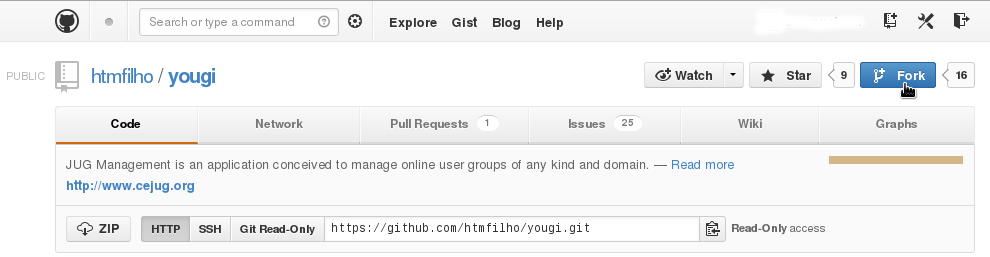
\includegraphics[height=3cm, angle=0]{figures/fork-yougi-github}
\caption{Clique em Fork}
\label{fig:1}
\end{figure}
\item Copie o URI do Fork recém criado e digite o seguinte comando para fazer o checkout do projeto: git clone https://github.com/[nome-de-usuario]/yougi.git. Ele vai criar uma pasta "yougi" no diretório que você executou o comando e o código fonte completo estará disponível lá.
\end{enumerate}

Para se certificar de que o código no branch do servidor está funcionando perfeitamente, temos que atualizar a cópia local com as últimas alterações disponíveis no servidor, testar o sistema localmente com essas mudanças e se tudo está funcionando bem, o commit local pode finalmente ser feito e o push para o seu respectivo branch. Antes de atualizar o local, certifique-se de que não há commit pendente usando:
\begin{verbatim}
# git status
\end{verbatim}
Se existem arquivos alterados adicioná-los usando:
\begin{verbatim}
# git add [arquivo]
\end{verbatim}
Use o comando acima para cada arquivo modificado ou se todos eles fazem sentido para ser commitados em conjunto usar:
\begin{verbatim}
# git commit -a -m “[mensagem]”
\end{verbatim}
para adicionar todos os arquivos alterados e commitar logo depois. Se os arquivos foram adicionados individualmente use:
\begin{verbatim}
# git commit -m “[mensagem]”
\end{verbatim}
Depois de realizar o último comete, é hora de atualizar a cópia local usando:
\begin{verbatim}
# git pull
\end{verbatim}
or
\begin{verbatim}
# git fetch
# git merge FETCH_HEAD
\end{verbatim}

Para empurrar o commit local para o servidor, utilize:

\begin{verbatim}
#git push origin master
\end{verbatim}

\subsection{Configurando e Construindo a Aplicação com Apache Maven}
	
\subsubsection{Ciclo de vida de construção}

\begin{enumerate}
	\item process-resources (processar recursos)
 	\item compile (compilar)
	\item process-test-resources (processar recursos de teste)
	\item test-compile (testar compilação)
	\item test (testar)
	\item package (empacotar)
	\item install (instalar)
	\item deploy (implantar)
\end{enumerate}
	
Para instalar o Maven acesse o site http://maven.apache.org/download.cgi baixe o arquivo apache-maven-3.0.5-bin.zip, após concluir a instalação descompacte o arquivo. Mova a pasta descompactada para dentro da pasta ''Arquivos de Programas'' (opcional);

\subsubsection{Configurando as Variáveis de Ambiente}

\begin{enumerate}
\item Clique com o botão direito no ícone ''Meu Computador” > “Propriedades”.
\item Clique em “Configurações avançadas dos sistemas”, na nova aba clique em “Avançada” > Clique no botão  "Variáveis de Ambiente";
\item Na lista, variáveis do sistema clique no botão "Novo..." para criar uma nova variável.
\item Digite no campo ''Nome da variável'' MAVEN\_HOME e no campo 'Valor da variável' digite o diretório do seu arquivo C:/Arquivos de programas/apache-maven-3.0.4 - ''OK'';
\item Selecione a variável "Path" na lista de "Variáveis do Sistema" e clique no botão "Editar";
\item No final do Valor da variável Digite > ;%MAVEN_HOME%\bin > no final do campo. (não se esqueça do ponto e vírgula (;));
\item Clique no botão "OK" > "OK".
\end{enumerate}

\subsubsection{Testando no Prompt de comando}

Abra o Prompt digite mvn –version
Se sua configuração estiver correta vai aparecer à versão do Maven que foi instalado no windows.
 
 	Possível ERRO
Em caso do erro “'mvn' não é reconhecido como um comando interno ou externo, um programa operável ou um arquivo em lotes ” verifique a configuração das variáveis se estão correta de acordo com o seu diretório do apache-maven.

\subsubsection{Instalando o Maven no Eclipse}
	Acesse o menu do Eclipse, Help > Eclipse MarketPlace > no campo Find digite “Maven” > “GO”. Aparecerá varias opções de Maven para downloads procure pelo o Maven “Maven Integration for Eclipse” clique no botão Install para fazer à instalação, depois de concluída a instalação, o Eclipse vai pedir para reiniciar.
	Depois da reinicialização do eclipse verifique se está com um caractere 'M' em cima do projeto Yougi, caso nao esteja clique com o botão direito em cima do projeto "Configure" > Convert to Maven.

\subsection {Testando o Maven no Eclipse}

Clique com o botão direito em cima do Projeto “Yougi” Run as > Maven Install, para compilar o projeto pelo o Maven. 

\subsection {Testando o Maven no Prompt de controle}

Acesse a pasta do projeto “Yougi” pressione Shift e clique com o botão direito em cima da pasta, clique em “Abri janela de comando aqui” e digite no prompt “Mvn clear Install –U”

\part*{Apêndice}

\chapter*{Propriedades do JavaMail}

Tabela da \ref{tab:javamail-properties} lista todas as propriedades do JavaMail relevantes.

\begin{table}
\centering
\caption{Lista completa de propriedades do JavaMail}
\label{tab:javamail-properties}
\begin{tabular}{lll}
\hline\noalign{\smallskip}
Nome & Tipo & Descrição  \\
\noalign{\smallskip}\hline\noalign{\smallskip}
mail.smtp.user & String & Nome de usuário padrão para o SMTP. \\
mail.smtp.host & String & Servidor SMTP para conectar. \\
mail.smtp.port & int & A porta do servidor SMTP para conectar-se.\\ & & Padrão para 25. \\
mail.smtp.connectiontimeout & int & Valor de tempo limite de conexão do socket em \\ & & milissegundos. O padrão é tempo limite infinito.\\
mail.smtp.timeout & int & Socket E/S valor de tempo limite em milissegundos. \\ & & O padrão é tempo limite infinito. \\
mail.smtp.from & String & Endereço de e-mail para usar o SMTP MAIL \\ & & comando. Isso define o retorno envelope \\ & & endereço. Padrão para msg.getFrom() ou \\ & & InternetAddress.getLocalAddress(). \\
mail.smtp.ssl.enable & boolean & Se setado para true, usa SSL para conectar e usar \\ & & a porta SSL por padrão. O padrão é false \\ & & para o protocolo "smtp" e true para o \\ & & protocolo "smtps". \\
mail.smtp.starttls.enable & boolean & Se true, permite o uso do STARTTLS\\ & & comando (se suportado pelo servidor) para\\ & & mudar a ligação a um TLS-protected\\ & & conexão antes de emitir qualquer login\\ & & comandos. Padrão para false. \\
mail.smtp.starttls.required & boolean & se true, requer o uso do STARTTLS \\ & & comando. Se o servidor não suporta a \\ & & STARTTLS command, ou o comando \\ & & falhas, o método de conexão irá falhar. \\ & &Padrão para falso. \\
\noalign{\smallskip}\hline
\end{tabular}
\end{table}

\backmatter

\printindex

\end{document}